 % !TEX root = ../report.tex
\section{Mobile application} 

\begin{figure}[H]
 \makebox[\textwidth][c]{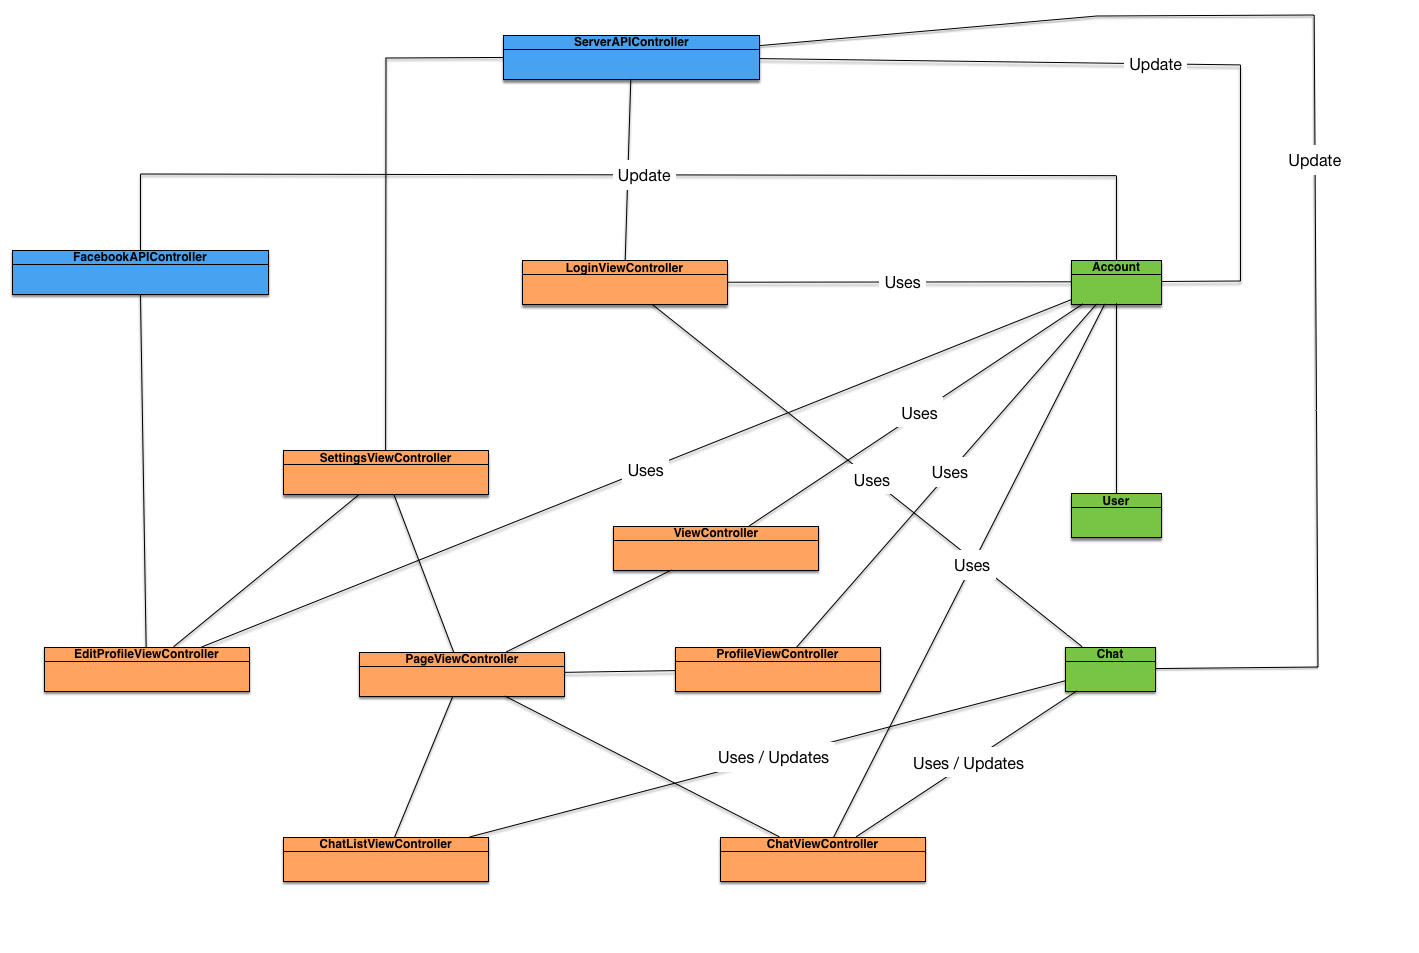
\includegraphics[width=1.6\textwidth]{./images/Tinfinity_general_class_diagram.png}}%
\caption{Simplified class diagram}
\end{figure}



The above class diagram shows a simplified version (only the most important classes are shown) of the application. The mobile application is based on eight main ViewController which handle the functionalities provided by Tinfinity:
\begin{itemize}
\item \textbf{LoginViewController} : Provides the login with Facebook functionalities and updates the account informations
\item \textbf{ViewController} : Provides to the user a map that shows where the other user are located and their profiles.
\item \textbf{SettingViewController} : Provides a recap view of the informations about the user and the ability to change them.
\item \textbf{EditProfileViewController} : Provides the functionalities to decide which photos have to be displayed.
\item \textbf{ProfileViewController} : Provides a view that shows the profile of other users which have sent a friendship request, and the abilities to accept / decline it.
\item \textbf{ChatListViewController} : Provides a view with a list of the chat and the provides the functionalities to delete them.
\item \textbf{ChatViewController} : Provides a view with the conversation with the specified user and the ability to send messages.
\item \textbf{PageViewController} : Manages all the other views. It doesn't provide any functionality to the user, but it is used only for internal purposes.
\end{itemize}  

\subsection{LoginViewController} 
\begin{figure}[H]
 \makebox[\textwidth][c]{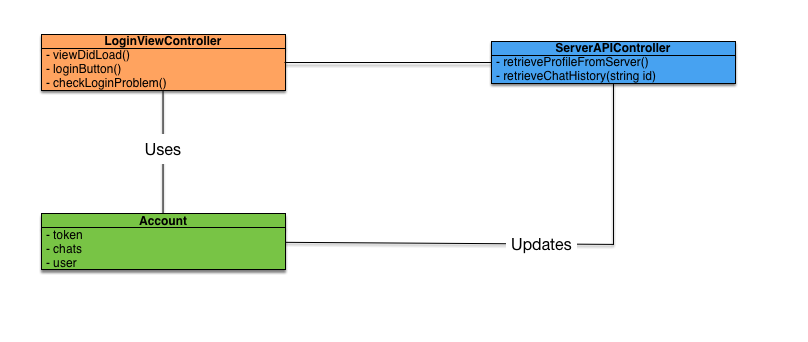
\includegraphics[width=1.6\textwidth]{./images/Tinfinity_LoginViewController.png}}%
\caption{LoginViewController class diagram}
\end{figure}

The LoginViewController manages the view that implement the login functionalities with Facebook and set up the initial settings relative to the account.

\begin{itemize}
\item \textbf{viewDidLoad()} : When the view is loaded this callback tries to check if there is already a valid Facebook OAuth token binded to the account. If the token is present and valid then the application will display the main view of the application.
\item \textbf{loginButton()} : This function is triggered when the login button is pressed. This function exploit the Facebook SDK in order to retrieve a valid OAuth token. If this operation succeed, then the other account settings, like the chat history, are retrieved and set and the main view of the application is displayed.
\end{itemize}


\subsection{ViewController} 
\begin{figure}[H]
 \makebox[\textwidth][c]{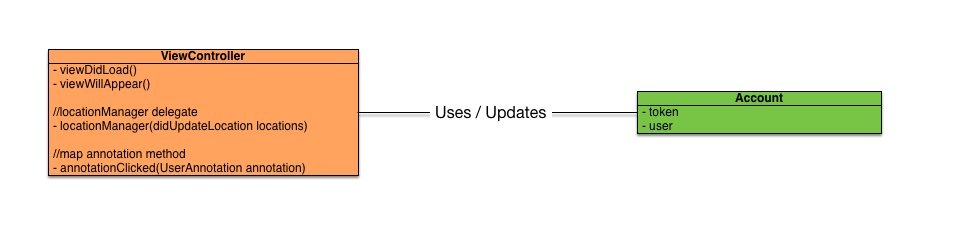
\includegraphics[width=1.6\textwidth]{./images/Tinfinity_ViewController.png}}%
\caption{ViewController class diagram}
\end{figure}


The ViewController manages the main view of the application and it show the map with the user location and the location of the other users around him. It is the delegate for the location manager and the mapView callback functions.

\begin{itemize}
\item \textbf{viewDidLoad()} : When the view is loaded this callback checks if the permissions needed in order to locate the user properly are given. if these are not given the map is hidden, otherwise the map is displayed and the user location is retrieved.
\item \textbf{viewWillAppear()} : Every time the view is shown the location of the user is updated.
\item \textbf{locationManager(didUpdateLocations error)} : Set the latitude and longitude of the user and add a marker on the map.
\item \textbf{annotationClicked(UserAnnotation annotation)} : When a marker of another is clicked the information relative to him are retrieved and passed to the ProfileViewController
\end{itemize}

\subsection{SettingsViewController} 
\begin{figure}[H]
 \makebox[\textwidth][c]{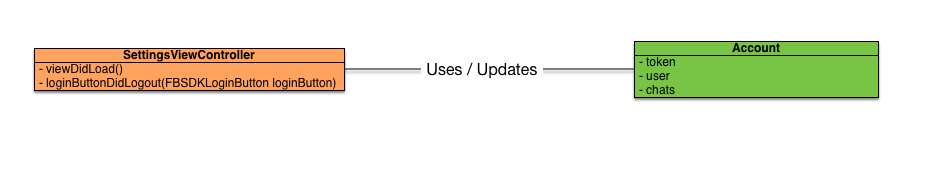
\includegraphics[width=1.6\textwidth]{./images/Tinfinity_SettingsViewController.png}}%
\caption{SettingsViewController class diagram}

\end{figure}

The SettingsViewController shows a view with the recap of the user informations and implement the logout functionality.

\begin{itemize}
\item \textbf{viewDidLoad()} : When the view is loaded all the informations about the user, like the profile picture, are retrieved and displayed properly.
\item \textbf{loginButtonDidLogout()} : Exploit the Facebook SDK in order to invalidate the OAuth token and log out the user from the application.
\end{itemize}

\subsection{EditProfileViewController} 
\begin{figure}[H]
 \makebox[\textwidth][c]{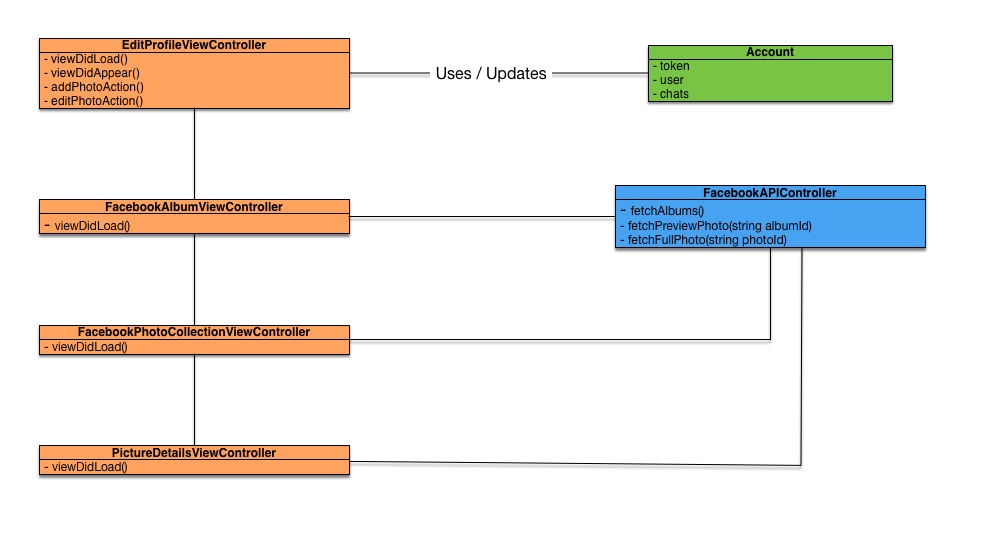
\includegraphics[width=1.6\textwidth]{./images/Tinfinity_EditProfileViewController.png}}%
\caption{EditProfileViewController class diagram}
\end{figure}


The EditProfileViewController and the other auxiliary ViewControllers (FacebookAlbumViewController, FacebookPhotoCollectionViewController and PictureDetailsViewController) provides the functionalities of the photo editing. The user here can decide which photos of his Facebook profile have to be displayed in the application.

\begin{itemize}
\item \textbf{viewDidLoad() (FacebookAlbumViewController)} : Fetches the Facebook photos album relative to the user.
\item \textbf{viewDidLoad() (FacebookPhotoCollectionViewController)} : Fetches the preview of the photos that are in the selected album.
\item \textbf{viewDidLoad() (PictureDetailsViewController)} : Fetches the high resolution version of the selected photo.
\end{itemize}


\subsection{ProfileViewController} 

\begin{figure}[H]
 \makebox[\textwidth][c]{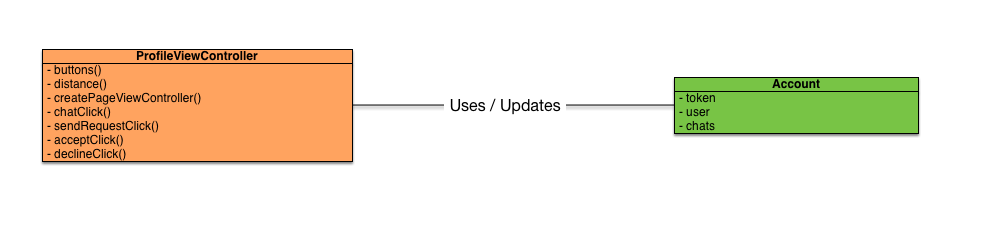
\includegraphics[width=1.6\textwidth]{./images/Tinfinity_ProfileViewController.png}}%
\caption{ProfileViewController class diagram}
\end{figure}


The ProfileViewController manages the view displayed when the user click on a marker on the map or when he receive a friendship request. This view shows all the details relative to the other user like the distance, his photos and his name and age. It provides also the functionalities in order to accept or decline a friendship request, send a new request, or start a new chat with the selected user.

\begin{itemize}
\item \textbf{buttons()} : Based on the relationship with the other user, this function decides which buttons have to be displayed.
\item \textbf{distance()} : This functions calculate the distance between the user and the other selected user.
\item \textbf{createPageViewController()} : Creates the photos slideshows with the photos of the other user.
\item \textbf{chatClick()} : Start a new chat with the other user.
\item \textbf{sendRequestClick()} : Send a friendship request to the other user.
\item \textbf{acceptClick() / declineClick()} : accept / decline a received friendship request.
\end{itemize}


\subsection{ChatListViewController} 

The ChatListViewController implements the application logic that takes care of these two thing:

\begin{enumerate}
\item Shows all the chat that the user has begun
\item Shows all the pending friendship request
\end{enumerate}

It also provides different functionalities based on the relationship between the two users. If they are friend it is possible to revoke the friendship status or delete the chat, if they are not it is possible to accept or decline the request or delete the chat.

\begin{itemize}

\item \textbf{viewDidLoad()} : Configure the table view that will handle the chat list and the binded actions

\item \textbf{tableView(editActionsForRowAtIndexPath indexPath: NSIndexPath)} : Set the proper action for each row:

\begin{itemize}
\item \textbf{accept} : set the status between the two user as "Friend" and sycronize it with the server
\item \textbf{decline} : send a request to the server in order to delete the friendship request
\item \textbf{request} : send a friendship request to te selected user
\item \textbf{unfriend} : delete the relationship between the users and synchronise it with the server

\end{itemize}

\item \textbf{updateData()} : refresh the information in the table view. this function is trigger when the user pull down the view

\end{itemize}

\subsection{ChatListViewController} 

The ChatViewController manages and display correctly the chat history between two users. Every message is displayed as a bubble, a blue one for the current user and a grey one for the other. It provides also the functionalities in order to send messages and updates the history when a new one is received.

\begin{itemize}

\item \textbf{viewDidLoad()} : Enables the chat only when the connection to the server is established
\item \textbf{toggleSend()} : Disable the send button if the connection to the server is interrupted. When the connection has been re-established, it re-enable the send button again. It disable the chat also if two users are not friend and the distance of the other is out of range (the distance between the two people are greater than 800m)
\item \textbf{didPressSendButton()} : Prepare the correct data structure for the message and send it. it also update the chat list appending the new message at the end of the list.
\end{itemize}

\subsection{Persistent Data Design}
\begin{figure}[H]
\centering
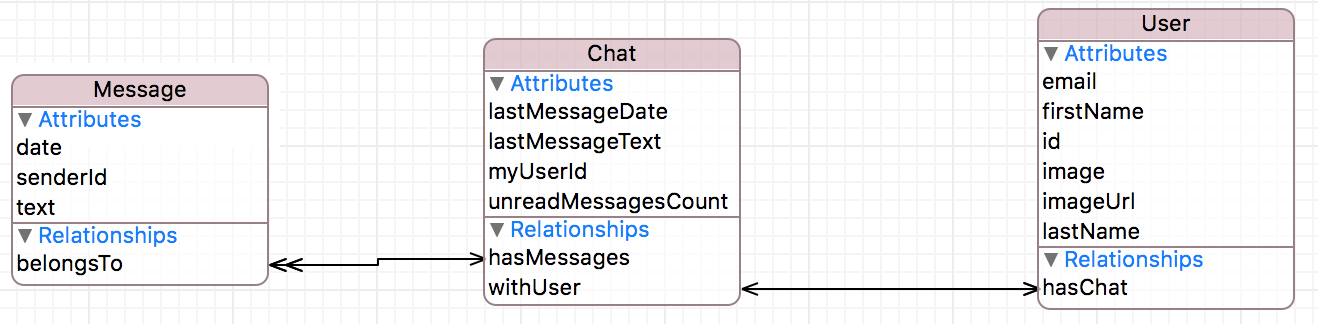
\includegraphics[width=1\textwidth]{./images/Tinfinity_CoreData.png}
\caption{Database}


The persistent Core Data is composed by 3 classes:

\begin{itemize}
\item \textbf{Message} : contains the informations of a single message(the date in which the message has been sent,the sender and the actual message text) and has a one-to-one relationship that associate it to a certain chat;
\item \textbf{Chat} : contains the information of a chat(the date and text of the last message that has been received, the id of the logged user and the counter of unread messages) and has two relationships, one is a one-to-many relationship with the message class, that associate the chat with all of his messages, and the other a one-to-one relationship with the User class, that represent the other user.
\item \textbf{User} : contains all the information of a user(email, name, surname, id, the user image and its url) and has a one-to-one relationship with the chat that is associated with it.
\end{itemize}
\end{figure}







